\documentclass[letterpaper,twocolumn,10pt]{article}

\usepackage[margin=1in]{geometry}
\usepackage[font=small]{caption}

\usepackage{listings}
\lstset{
   breaklines=true,
   basicstyle=\ttfamily}
\usepackage{graphicx}

\begin{document}

\title{Improving Qubit Measurement Reliability by Machine Learning Methods}

\author{Yingbo (Max) Wang}

\maketitle

\section{Abstract}

Quantum computing has bright prospects of domain-specific applications such as optimization, chemistry and machine learning, but the high-error rate of its computational unit - the qubit - has been a primary restricting factor. Regarding a qubit's State Preparation and Measurement (SPAM) reliability, this project focuses on the measurement part, explores multiple statistical and machine learning models used on the experimental data and determines the measurement accuracy of whether a given qubit is in the 0-state or a 1-state. The models, including Logistic Regression, Random Forest, Multilayer Perceptron and an emsemble of them, are applied on datasets of trapped-ion qubits from UCLA Physics that record the arrival timestamp of each reflected photon in the measurement experiment. The baseline model which performs classification by counting the number of captured photons achieves an accuracy of 99.97081\%. With a Multilayer Perceptron neural network model with careful input feature selection and hyper-parameters tuning, we are able to achieve a measurement accuracy of 99.97934\% with a random training and testing data split, which is close to the theoretical maximum at 99.98\%. In addition, we propose alternative methods to train the model and evaluate its performance and methods to split training and testing data, with the goal to minimize bias in performance evaluation and maximize the outcome in model's learning. With these new methods, the best-performing model is evaluated at an accuracy of 99.97236\%. It's still an improvement over the baseline and the accuracy is more likely to pertain in future datasets. Lastly multiple apporaches are discussed that are worth exploring in the next stage of this project.

\section{Introduction}

Quantum computing has promising prospects of applications in domain-specific computational-intensive tasks - for example, in the field era of optimization, chemistry, machine learning and cryptography \cite{quantum-application}. As a fast-growing research area, the computational power of available quantum computers approximately doubles every month: Google AI in partnership with NASA has claimed to have achieved quantum supremacy in October 2019 \cite{google-ai}, which implies a quantum computer is capable of solving a problem that none of the available classical computers practically can due to performance constraints. Qubits are the fundamental computational units in quantum computers, which are analogous to Bits in classical computers. Following rules of quantum mechanics, each qubit can be in a 0-state, a 1-state or any state that is a superposition of these two states. Multiple qubits in the same system are interacting with each other creating a state of entanglement, so only the state of the system can be described but not each individual qubit. The superposition and entanglement properties of qubits allow the quantum computer to double its computational ability for every qubit added, and thus contribute to the potential of its high performance growth. A qubit falls to either the 0-state or 1-state during measurement, where its previous state determines the probability of falling into each. 

However, current quantum computers has a major drawback compared to classical computers: the error rate of a qubit is magnitudes higher than its classical counterpart. These are referred to as Noisy Intermediate-Scale Quantum Computers and potential applications are significantly limited until the error rate can reduced \cite{quantum-application}. One approach to this problem is to build fault-tolerant logical qubits on top of physical qubits \cite{fault-tolerance}. It's not pratical in the near future because fault-tolerance in a quantum system is much more expensive than in a classical system, where an error-free logical qubit takes hundreds of actual physical qubits to build. Our project aims to mitigate the problem from another perspective which improves reliability of each individual physical qubit. Factors that reduce a qubit's reliability consist of preparation errors, where the qubit is not physically initiated to the desired state, and measurement errors, where the measurement does not correctly determine the state that the qubit falls to. As state preparations have already achieved high reliability, this project focuses on reducing the measurement error by applying Machine Learning methods on the physical experiment results.

In particular, the dataset is gathered from the UCLA Physics department which is claimed to be capable of generating the most reliable qubit in the world, with State Preparation and Measurement (SPAM) Reliability greater than 99.97\%. To measure such a trapped-ion qubit, a beam of photons are shooted at the target qubit at $t = 0$ while a receptor starts capturing photons reflected back from the target. A list of timestamps is recorded of the arrival times of each photon captured. The pattern of the number of photons captured and their timestamps is expected to be different depending on the difference of the particles' energy levels when the qubit is at the 0-state or the 1-state. Thus, given the above information of captured photons in the experiment, the goal of this project is to determine the measurement accuracy by exploring multiple statistical and machine learning models on the dataset, so that the optimal approach can be applied for a better measurement reliability. 

\section{Baseline Model}

\subsection{Basic Threshold Cutoff}

On the level of data processing with the details of physics abstracted away, the task is essentially a classification problem with two target labels: the 0-state or Bright state and the 1-state or Dark state. A dataset of about 387,000 instances is provided with a similar number of Bright instances and Dark instances, (194,000 Bright instances, 193,000 Dark instances) and used in all of the following experiments. We started with a verification of a basic baseline model that classifies a qubit based on the total number of photons captured. As an observation of the given dataset, qubits in the Bright state tend to result in significantly more captured photons than qubits in the Dark state, so it becomes reasonable that this model may give acceptable results. The cutoff threshold value is the only hyper-parameter to tune in this model: we tested all possible values ranging between 0 and 77 (the most number of photons captured when measuring one single qubit in our dataset) and selected the value that offers the best performance. Accuracy of classification (the percentage of correctly-classified instances over all tested instances) is a reasonable and intuitive metric for measuring model's performance in our application, so we used it in this and all following experiments. This model does not have any internal parameters to be tuned, so no split of training/testing instances is necessary in the dataset and all instances can be used to best evaluate the model's performance.

Figure \ref{fig:threshold_cutoff} shows the accuracy of each tested threshold value with some notable values listed in Table \ref{table:threshold_cutoff}. Value 12 achieves the best accuracy in our dataset, where the model classifes a qubit as Bright if more than 12 photons are captured and as Dark otherwise. The baseline model with this hyper-parameter achieves an accuracy of 99.97081\%, which is later referred as the baseline performance and compared with. As an observation from the graph, the model with threshold values between 7 and 18 all achieve pretty similar and high accuracy greater than 99.9\%. This fact implies that the model hasn't been able to utilize additional information inside these captured photons. A more complex statistical or machine learning model may be able to learn this information and yield better performance. 

\begin{table}
    \caption{Reliability of Threshold Cutoff Model at different count thresholds}
    \begin{center}
        \begin{tabular}{c c}
            Count Threshold & Accuracy \\ [0.5ex] 
            \hline
            5 & 99.497\% \\ 
            10 & 99.969\% \\
            15 & 99.967\% \\
            20 & 99.837\% \\
            25 & 98.748\% \\
       \end{tabular}
    \end{center}
    \label{table:threshold_cutoff}  
\end{table}


\begin{figure}
    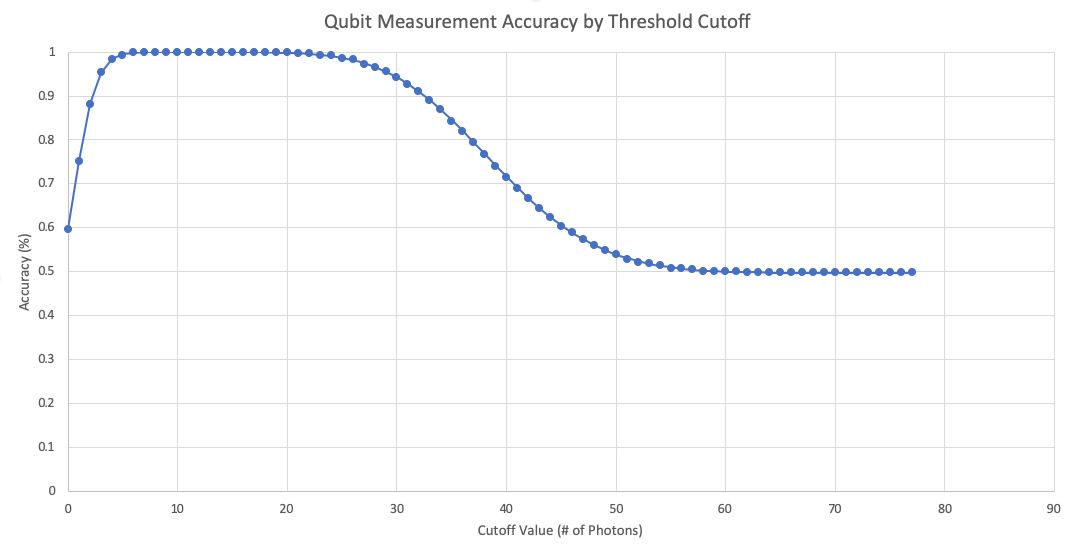
\includegraphics[width=\linewidth]{Figures/threshold_cutoff_accuracy.png}
    \centering
    \caption{Reliability of Threshold Cutoff Model}
    \label{fig:threshold_cutoff}
\end{figure}

\subsection{Threshold Cutoff with Early-Arrived Photons}

The paper by Seif, et al. aims to solve a similar, more complex problem that measures multiple qubits with readout crosstalk \cite{ml-qubit}, so its approaches are referenced and conditionally applied in our situation. As one of its methods, the classification accuracy may be improved by choosing an optimal timeframe of collecting photons. Additional photons may be captured late in time for Dark qubits due to off-resonant dark-to-bright pumping, so ideally the model would want to filter out those photons before making a decision. This model thus classifies a qubit by counting the number of photons captured within a certain timeframe before a pre-determined threshold. It has two hyper-parameters to tune: the count threshold value for total number of photons captured and the time threshold value for filtering out late-arrived photons. We tried all possible combinations of these two thresholds and evaluated the model's performance with similar methods described in the previous section. The time threshold starts from 5.29914 milliseconds (ms) (the latest-arriving photons among all instances in the dataset) and decreases to 0 (filtering out all photons) with a step of 0.1 ms.

Figure \ref{fig:threshold_cutoff_early_arrival} shows the accuracy on the z-axis with each hyper-parameter set specified in the x and y-axis. It demonstrates that ignoring a few latest-arrived photons while keeping a similar photons count threshold leads to the model's best performance. Table \ref{table:threshold_cutoff_early_arrival} shows the hyper-parameters that achieve these results: the accuracy slightly jumps from the baseline accuracy to 99.97107\% by removing 1 false negative or false positive instance.

\begin{figure}
    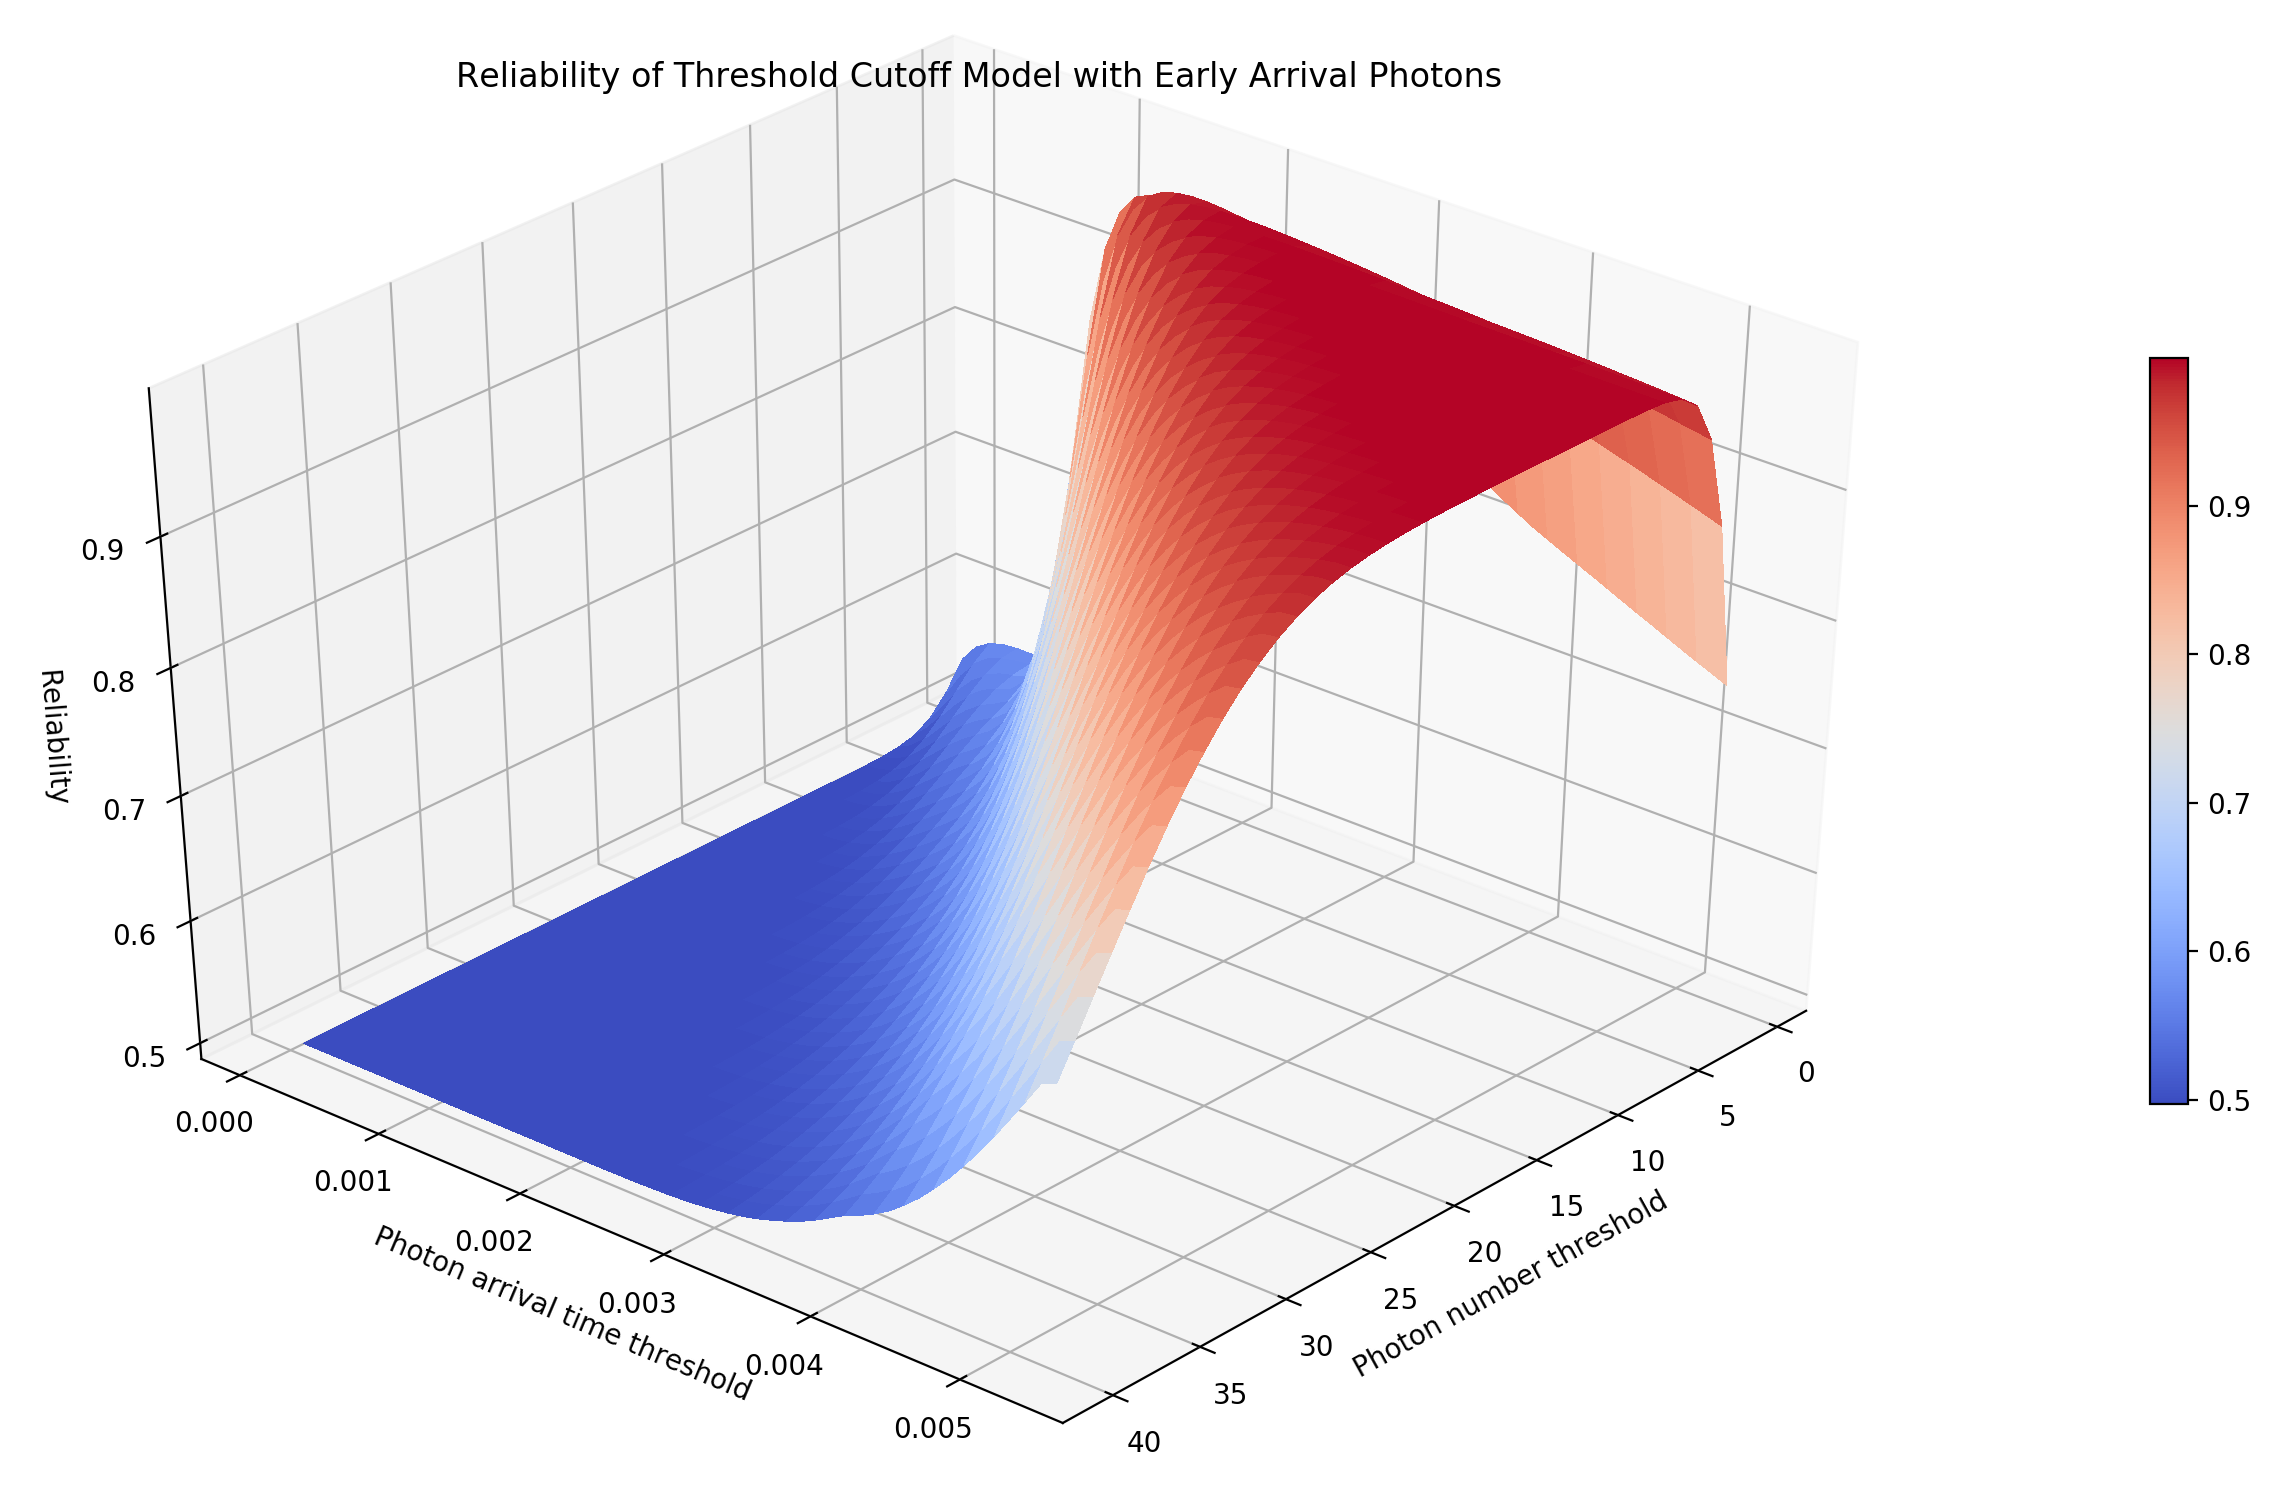
\includegraphics[width=\linewidth]{Figures/threshold_cutoff_early_arrival_accuracy.png}
    \centering
    \caption{Reliability of Threshold Cutoff Model with early-arrived photons}
    \label{fig:threshold_cutoff_early_arrival}
\end{figure}

\begin{table*}
    \caption{Reliability of Threshold Cutoff Model with Early-Arrived Photons at different count and timing thresholds}
    \begin{center}
        \begin{tabular}{c c c c c}
            Count Threshold & Timing Threshold & Accuracy & Number of False Positives & Number of False Negatives \\ [0.5ex] 
            \hline
            N/A	& 12 & 99.97081\% & 39 & 74 \\
            5.19914	ms & 12 & 99.97107\% & 39 & 73 \\ 
            5.509914 ms & 12 & 99.97107\% & 40 & 72 \\
            4.99914 ms & 11 & 99.97107\% & 39 & 73 \\
            4.99914 ms & 12 & 99.97107\% & 40 & 72 \\
       \end{tabular}
    \end{center}
    \label{table:threshold_cutoff_early_arrival}  
\end{table*}

Meanwhile, investigating the properities of the dataset confirms this result. Graph \ref{fig:distro_photons_arrival_times} shows a histogram illustrating the arrival times distribution of photons captured in all instances of the dataset. It's clearly seen that most photons arrive in three consecutive and disjoint time intervals where a few photons arrive in the fourth interval after the first three dominant intervals. The late arrived-time of these few photons may be explained by measurement errors so it's reasonable to ignore these photons in classification. Data shows the fourth interval starts at $t = 5.22625 \ ms$ which should be set as the model's timing threshold. This theoretical value corresponds with our experimental result above considering the precision restriction due to our coarse-grained step value.

\begin{figure}
    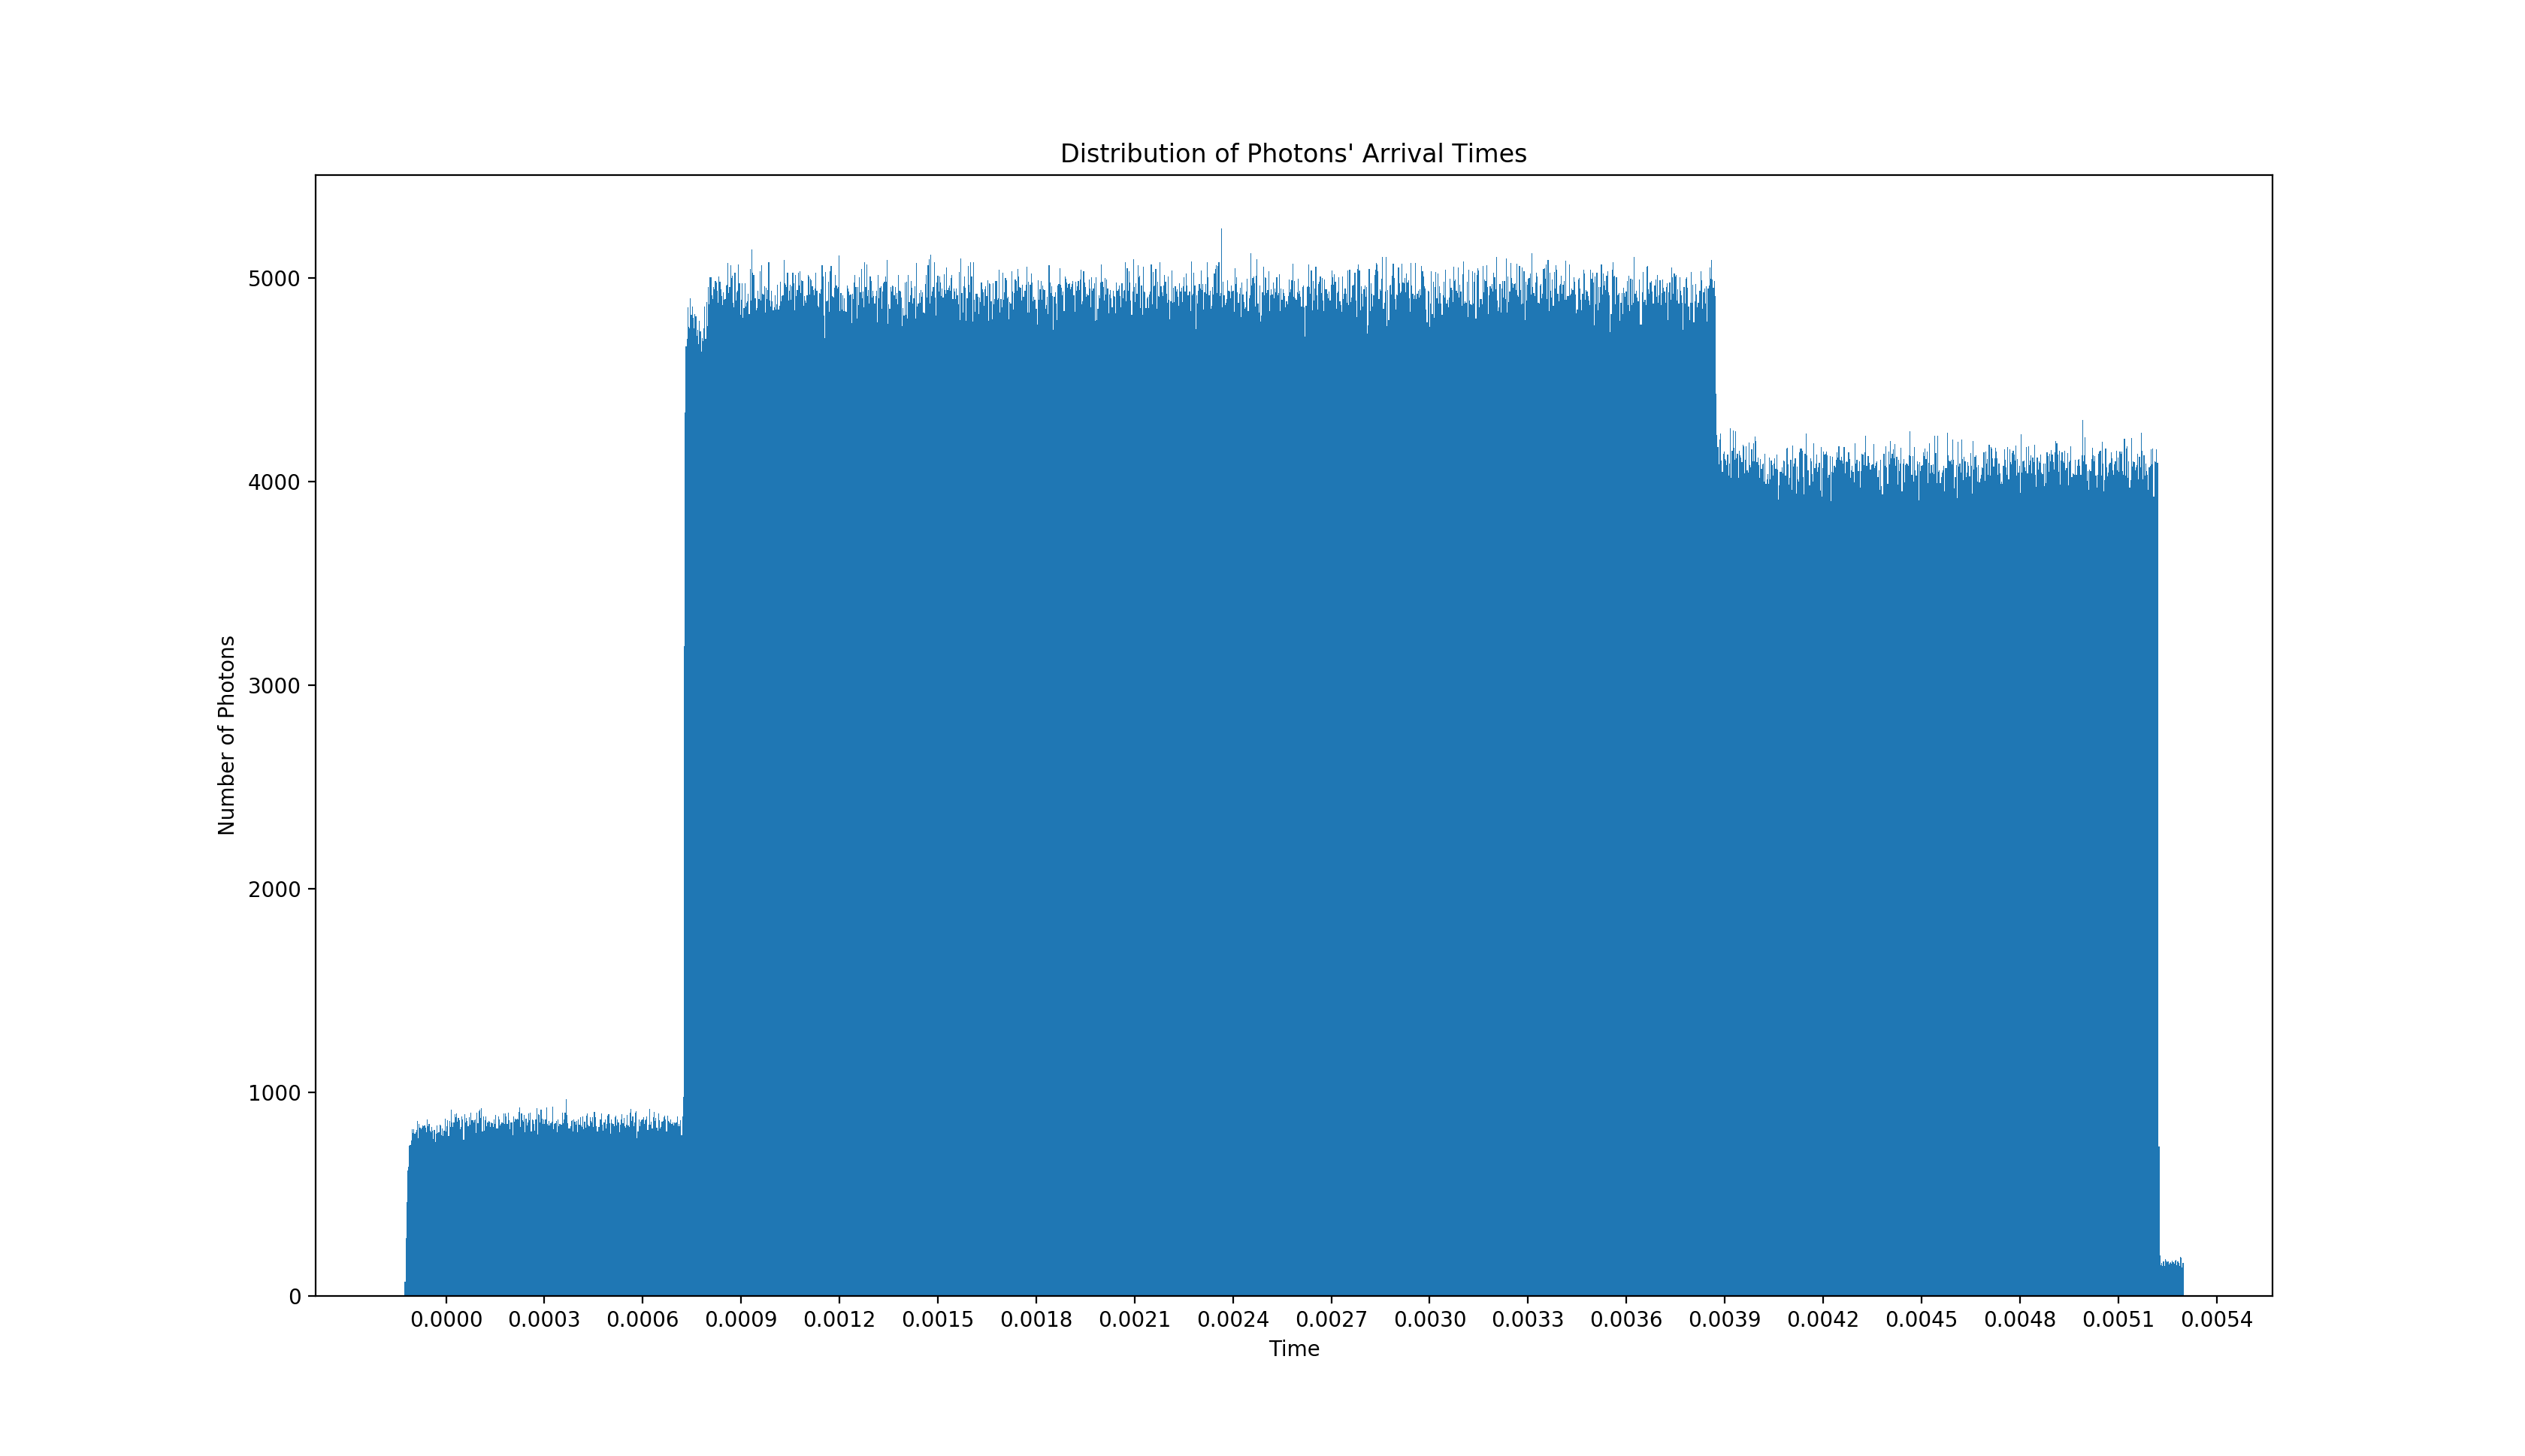
\includegraphics[width=\linewidth]{Figures/distro_photons_arrival_times.png}
    \centering
    \caption{Distribution of all photons' arrived times in the dataset as a histogram}
    \label{fig:distro_photons_arrival_times}
\end{figure}

\section{Machine Learning Models}

\subsection{Multilayer Perceptron}

We started exploring Machine Learning-based classification models afterwards with the hope to utilize more information provided in the timestamp of each captured photon. The Multilayer Perceptron (MLP) model is a classical type of feedforward artificial neural network (ANN): compared to traditional statistical models such as linear regression, neural network models are better at capturing non-linear and other more complex relations between the input features and the ouput target. These non-obvious, non-linear relations are the information we hope to utilize besides the approximately-linear relation between the number of photons captured and the target label, so such neural network models are a reasonable starting point. Graph \ref{fig:mlp_architecture} shows an example of a MLP model's architecture. The model consists of three or more layers of fully connected neurons, including one input layer, one or more hidden layers and one output layer. According to our model design, each neuron in the input layer takes one element in the input vector and each neuron in the output layer gives the probability of the qubit residing in a particular state. Each neuron denotes an arithmetic operation taking inputs $x_k$ and transforming to one output $f(\sum_{k}{w_k}{x_k} + b)$, where $f$ is the activation function of choice and $w_k, b$ are weights and bias of the neuron. The weights and bias of each neuron are the parameters of the model and the goal of training is to find the set of parameters that offer the best classification performance.

\begin{figure}
    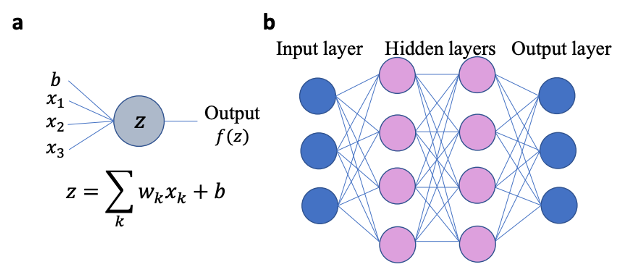
\includegraphics[width=\linewidth]{Figures/mlp_architecture.png}
    \centering
    \caption{Architecture overview of a Mutlilayer Perceptron model. Image credit: \cite{ml-qubit}}
    \label{fig:mlp_architecture}
\end{figure}

In particular, as a procedure of input feature selection, we took the histogram of the timestamps of captured photons in the instance over a pre-determined number of equally-sized intervals. This transformation ensures every instance has a consistent dimension as the input to the classification model regardless of the total number of captured photons. Thus, the number of input neurons in the MLP model equals the number of histogram bins; the number of output neurons always equals two as we're classifying one individual qubit with two possible states, where the sum of their output always equals 1 by probability theory. Following the result in the previous section, late-arrived photons arrived after 5.29914 ms are ignored. We used ReLU as the activation function where $f(x) = max(0, x)$: it preserves the original information for all non-negative values, which suits well for our use case where the photons' arrival timestamps are non-negative. Training is performed with the Adam optimizer based on the gradient descent method. As a typical choice of a classification model, Cross-Entropy is used as the loss function to evaluate the model's performance on a particular set of parameters: the optimizer iterates and converges to the set of parameters that minimizes the loss. The outputs in the last layer are normalized with a Softmax function to a range between 0 and 1 corresponding to the probabilistic interpretation, and a target class with the highest probability is selected.

As shown by Seif, et al., a network with 2 hidden layers and between 8 and 40 neurons per layer provides the best performance depending on the complexity of the application, so we experimented with all these hyper-parameters on the model and reviewed the result. The dataset is randomly split into 80\% training and 20\% testing instances with a randomly selected seed to ensure reproducibility. To avoid bias of evaluation, the testing set is not exposed until the best set of hyper-parameters is determined and is only used to evaluate the final performance of that final model. A 4-fold Cross Validation is used to measure the performance of each set of hyper-parameters without wasting any training data; the complete procedure that finds the best-performing hyper-parameters and evaluates the model's accuracy is outlined in Listing \ref{lst:separate-testing}. All of the above dataset split ensures the percentage of Dark instances and Bright instances is the same among all splits. This procedure of model training, testing and hyper-parameters tuning will be referred as Separate Testing Method later in the report for convenience. With this method, we found that using 32 neurons per layer yields the highest classification accuracy at 99.97934\%, with 12 false positives and 4 false negatives over 77427 testing samples. The result reached is close to the claimed theoretical maximum reliability that can be achieved on such a trapped-ion qubit, which is about 99.98\%.

\begin{lstlisting}[basicstyle=\scriptsize, float=*, label={lst:separate-testing}, caption={Pseudocode for the Separate Testing Procedure}]
Split 80% instances into the training set and 20% into the testing set
Split the training set into 4 equally-sized groups (each contains 20% of all available instances)
For each set of hyper-parameters:
    Initialize a list of accuracy values
    Repeat 4 times (with i = 1, 2, 3, 4):
        Leaves instances in Group i for testing and trains model on instances in the other 3 groups
        Test the model with instances in Group i and append the accuracy value to the list
    Find the model's accuracy by taking average of the 4 values in the list
Find the hyper-parameters that give the best averaged accuracy

Train a model with these hyper-parameters on all training instances
Test the model on testing instances and return the accuracy value
\end{lstlisting}

\subsection{Other Models}

In addition, we applied the Logistic Regression and Random Forest model which are both commonly used in general classification tasks. Logistic Regression, as a special case of the generalized linear model, is a statistical model that uses the logistic function to model a binary target variable by estimating probabilities of relations between the input features and the target. Random Forest is an ensemble learning method that constructs multiple decision trees during training and predicts the target by finding the mode prediction of individual trees. We used the same Separate Testing Method explained above to perform training and evaluation of each model. In particular, various hyper-parameters of the Logistic Regression model are tested and evaluated. Table \ref{table:ml_models} summarizes the hyper-parameters selection and the model's performance. It's seen that the performance is similarly or slightly below that of the Multilayer Perceptron model. We expect this to be due to the latter's better ability of capturing non-linear relations in the dataset.

\begin{table*}
    \caption{Accuracy of multiple Machine Learning classification methods}
    \begin{center}
        \begin{tabular}{c c c}
            Model & Best-performing Hyper-parameters & Accuracy \\ [0.5ex] 
            \hline
            Multilayer Perceptron & 32 neurons per layer & 99.97934\% \\
            Logistic Regression	& 
                \begin{tabular}{@{}c@{}} 
                    Regularization Strength C = 0.001, \\ l2 Regularization
                \end{tabular} 
            & 99.97934\% \\
            Random Forest & 100 Estimators/Trees & 99.97804\% \\ 
       \end{tabular}
    \end{center}
    \label{table:ml_models}  
\end{table*}

\section{Model Improvements}

After a deeper dive into our dataset, we realized two key factors that impact the performance of a given model. The discrepency in performance is not large by absolute value but is practically significant considering the small difference between the accuracy of our baseline model (about 99.97\%) and the theoretical maximum (about 99.98\%). In other words, any small improvement on accuracy may be meaningful in this situation, and extra care has to be taken to verify the statistical significance of the claimed accuracy and to increase precision.

\subsection{Fairer Evaluation Method}

The first factor is to apply a fair evaluation method for a given classification model to increase the precision of measured accuracy. In the previous Separate Testing Method, although the training and testing sets are split by random, bias of evaluation could result if the instances in the testing set possess patterns more or less regular. For instance, a testing set that's easier to predict than the dataset's average would lead to an over-estimation of the model's accuracy, and vice versa. Thus, a fairer method of perform model training and testing needs to be proposed so that it accounts for every instance in the dataset when evaluating the model. 

One such evaluation method is simply an extension to the Separate Testing Method, called Separate Testing Method Extension, by repeating the procedure multiple times and taking the averaged accuracy of all procedures. The dataset is evenly separated into 5 sets during the initial training/testing set split. The procedure is performed 5 times with instances in one set chosen for testing and those in the other 4 for training. This method theoretically gives a fairer evaluation of a model's accuracy; however, it would be difficult to conclude on the best hyper-parameters of the best given model, because the parameter tuning procedure may report at most 5 different values when it's repeated on different training instances. Also, the total time required for evaluation increases by a factor of 5 for one set of hyper-parameters of a model, making hyper-parameter tuning in a larger space less efficient.

These drawbacks motivate us to propose a simplified version of the above method, called Cross Testing Method. Instead of cross validating each set of hyper-parameters on the training set, the model directly performs training and testing over splits of the entire dataset and takes the averaged accuracy from every iteration. The pseudocode in Listing \ref{lst:cross-testing} below outlines this procedure and Figure \ref{fig:testing_methods} compares the three training \& testing procedures described above. The removal of the separate testing set does not cause a loss of equity or generality of model evaluation, and the new method takes about the same time to run as the original Separate Testing Method given the same input. We have tested the Separate Testing Method Extension and the Cross Testing Method on the parameters tuning in Section 4.1: the reported accuracy is simlar, which is an experimental result confirming the the effectiveness of the new method.

\begin{figure}[]
    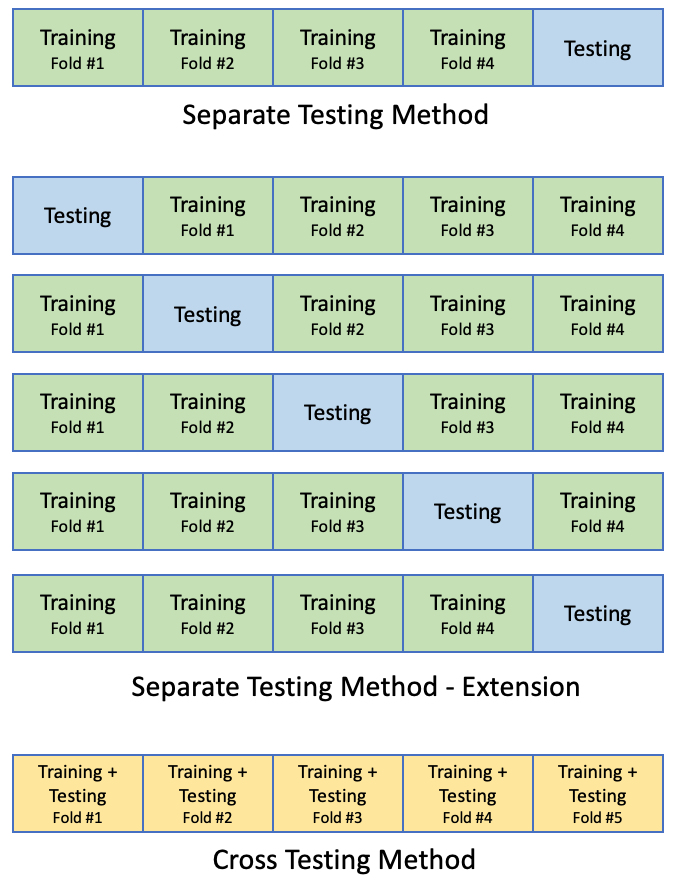
\includegraphics[width=\linewidth]{Figures/testing_methods.png}
    \centering
    \caption{Summary of the three model evaluation methods. Hyper-parameters tuning and selection is performed per row, using every fold in that row with a Cross Validation approach.}
    \label{fig:testing_methods}
\end{figure}

\begin{lstlisting}[basicstyle=\scriptsize, float=*, label={lst:cross-testing}, caption={Pseudocode for the Cross Testing Procedure}]
Split the training set into 5 equally-sized groups (each contains 20\% of all available instances)
For each set of hyper-parameters:
    Initialize a list of accuracy values
    Repeat 5 times (with i = 1, 2, 3, 4, 5):
        Leaves instances in Group i for testing and trains model on instances in the other 4 groups
        Test the model with instances in Group i and append the accuracy value to the list
    Find the model's accuracy by taking average of the 5 values in the list
Find the hyper-parameters that give the best averaged accuracy and return the accuracy value
\end{lstlisting}

\subsection{Training/Testing Dataset Split}

In addition, various key properties in the dataset should be kept consistent between each set of training and testing instances. Such consistent distributions ensure the model is always exposed to typical data instances of the application. The model would thus be able to learn the most number of patterns from training and evaluation bias would be best prevented in testing as explained above. Some of these properties include:

\begin{itemize}
    \item Percentage of Bright qubits and Dark qubits (already considered in Section 4.1)
    \item Distribution of arrival times of all captured photons
    \item Distribution of the number of Bright and Dark qubit instances for any particular number of photons captured
\end{itemize}

Figure \ref{fig:datasplit_good} shows an example of a reasonable dataset split. Here we assume the Cross Testing Method is used for evaluation, where the dataset is split into 5 folds and each evaluation's iteration involves a training set and a testing set. The left graph shows the distributions of all photons' arrival times have a very similar shape of three distinct regions in three similar timeframes. The right graph looks at the training and testing set of the 1st fold data split for demonstration: it shows the distribution of qubit instances is simlar among the number of photons captured between the training and the testing dataset, for both the Bright and Dark qubits. Particularly, most Dark qubits capture less than 10 photons and are thus cluttered on the left, while most Bright qubits capture a number of photons distributed almost normally centered at slightly less than 40 photons. This observation corresponds with the rationale behind the Threshold Cutoff Model explained in Section 3.1. 

Meanwhile, a bad dataset split tends to generate misleading evaluation results of a model, with one example shown in Graph \ref{fig:datasplit_bad}. This random split guarantees none of the consistency requirements outlined above; the graph shows that while the training set looks to have reasonable distributions, the testing set contains mostly Bright qubits. With such a testing set and the Separate Testing Method of evaluation, the baseline Threshold Cutoff Model with threshold at 12 photons can achieve accuracy of about 99.99\%, even higher than the theoretical maximum reliability. However, this high accuracy value does not imply a better performing model, but simply an easy-to-predict testing set that adds bias to our model evaluation procedure.

\begin{figure*}[]
    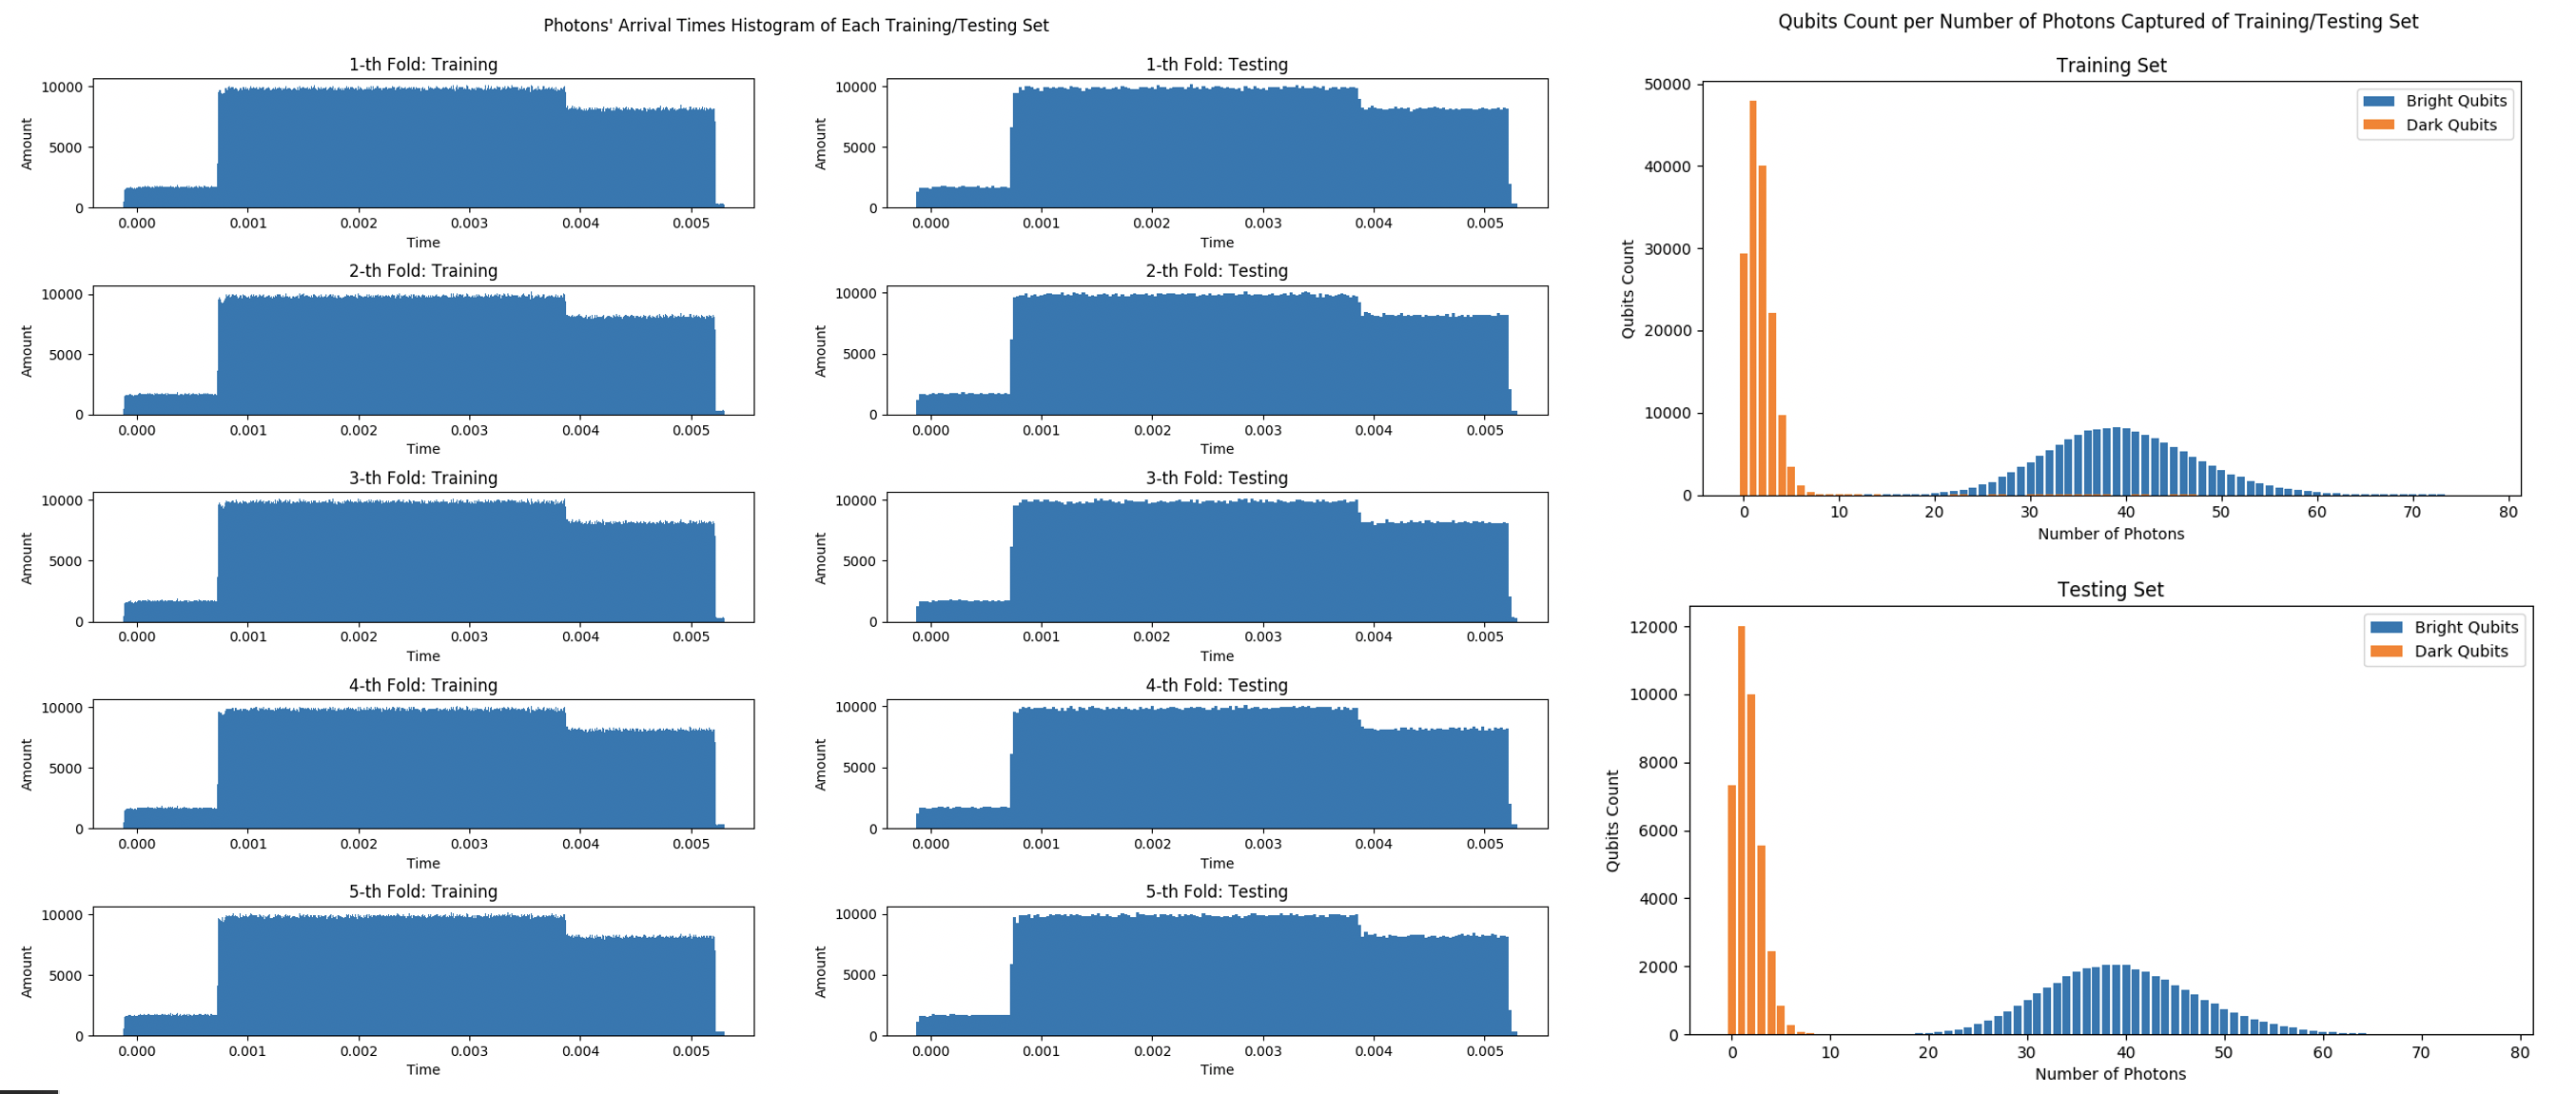
\includegraphics[width=2\columnwidth]{Figures/datasplit_good.png}
    \centering
    \caption{Example of a reasonable dataset split}
    \label{fig:datasplit_good}
\end{figure*}

\begin{figure}[]
    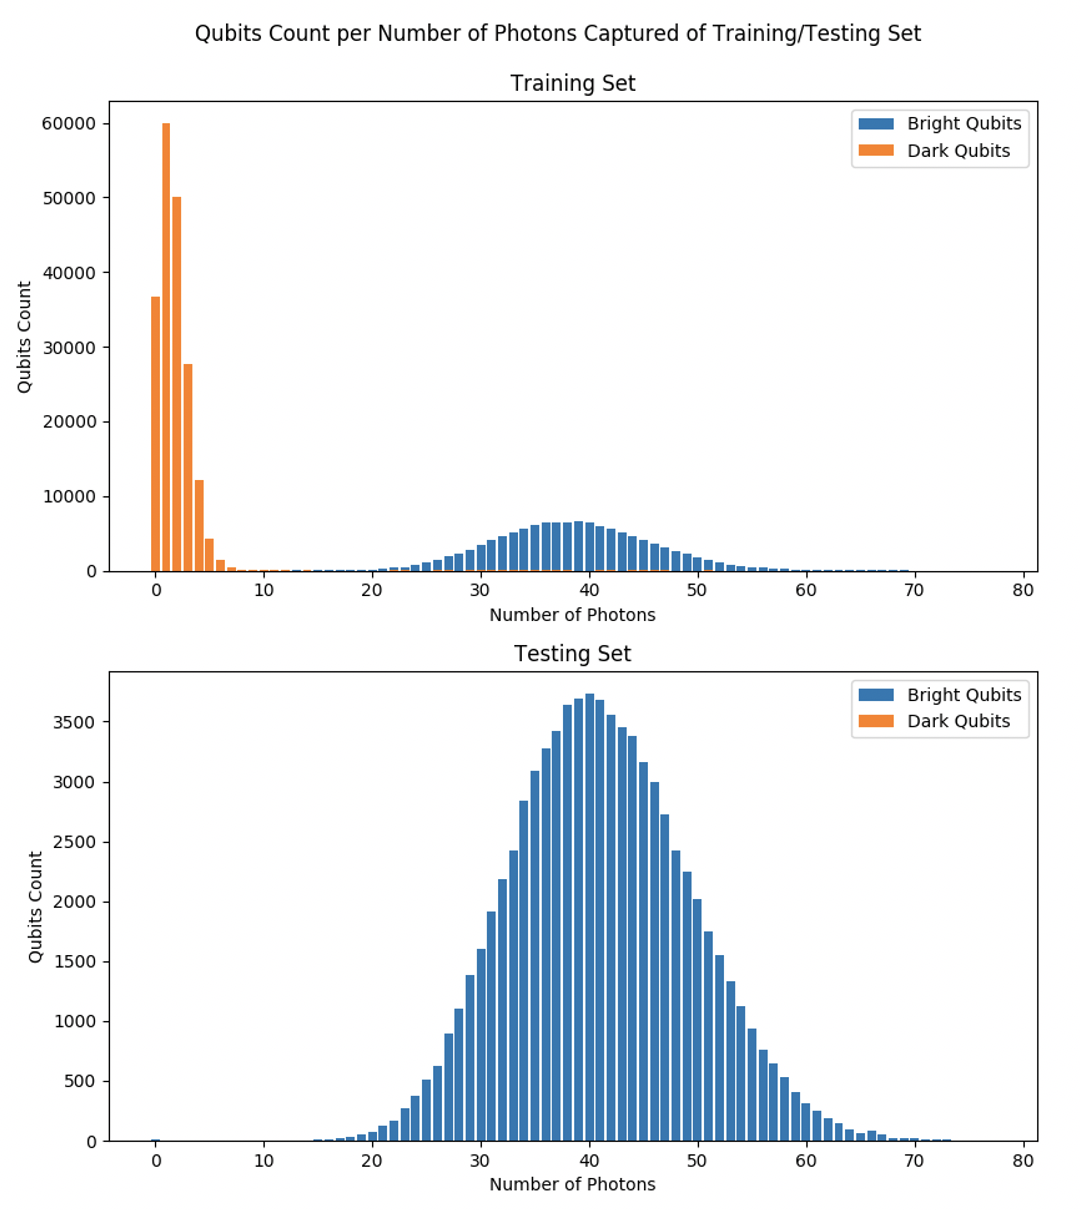
\includegraphics[width=\linewidth]{Figures/datasplit_bad.png}
    \centering
    \caption{Example of a misleading dataset split}
    \label{fig:datasplit_bad}
\end{figure}

\section{Results and Analysis}

\subsection{Hyper-parameters Tuning}

With the above Cross Testing Method of model evaluation and a proper data split, we performed training and testing of the Multilayer Perceptron model described in Section 4.1 with various set of hyper-parameters. The complete classification task is performed with a data Pipeline of two stages: a \texttt{Histogramizer} that pre-processes input photons' arrival time data and creates histograms, and a \texttt{MLPClassifer} that performs classification with the neural network. The classification model is implemented with the \texttt{scikit-learn} library in Python. The hyper-parameters being tuned in this Pipeline are:

\begin{itemize}
    \item Timestamp threshold to ignore photons arrived too early or too late
    \item Number of input histogram bins for captured photons
    \item Number of layers in the MLP model
    \item Number of neurons per layer in the MLP model
\end{itemize}

The evaluation results are summarized in Table \ref{table:params_tuning}. The best accuracy is achieved at 99.97236\%, which is slightly below the performance reported in Section 4.1 with the Separate Testing Method. This revised accuracy value should be seen as a more objective evaluation of the model's performance because the Cross Testing Method has accounted for all easier-to-predict and harder-to-predict instances. Under this new evaluation, we have still gained a performance improvement over the baseline model and are more confident that the same level of performance can be achieved on future datasets. 

\begin{figure*}[]
    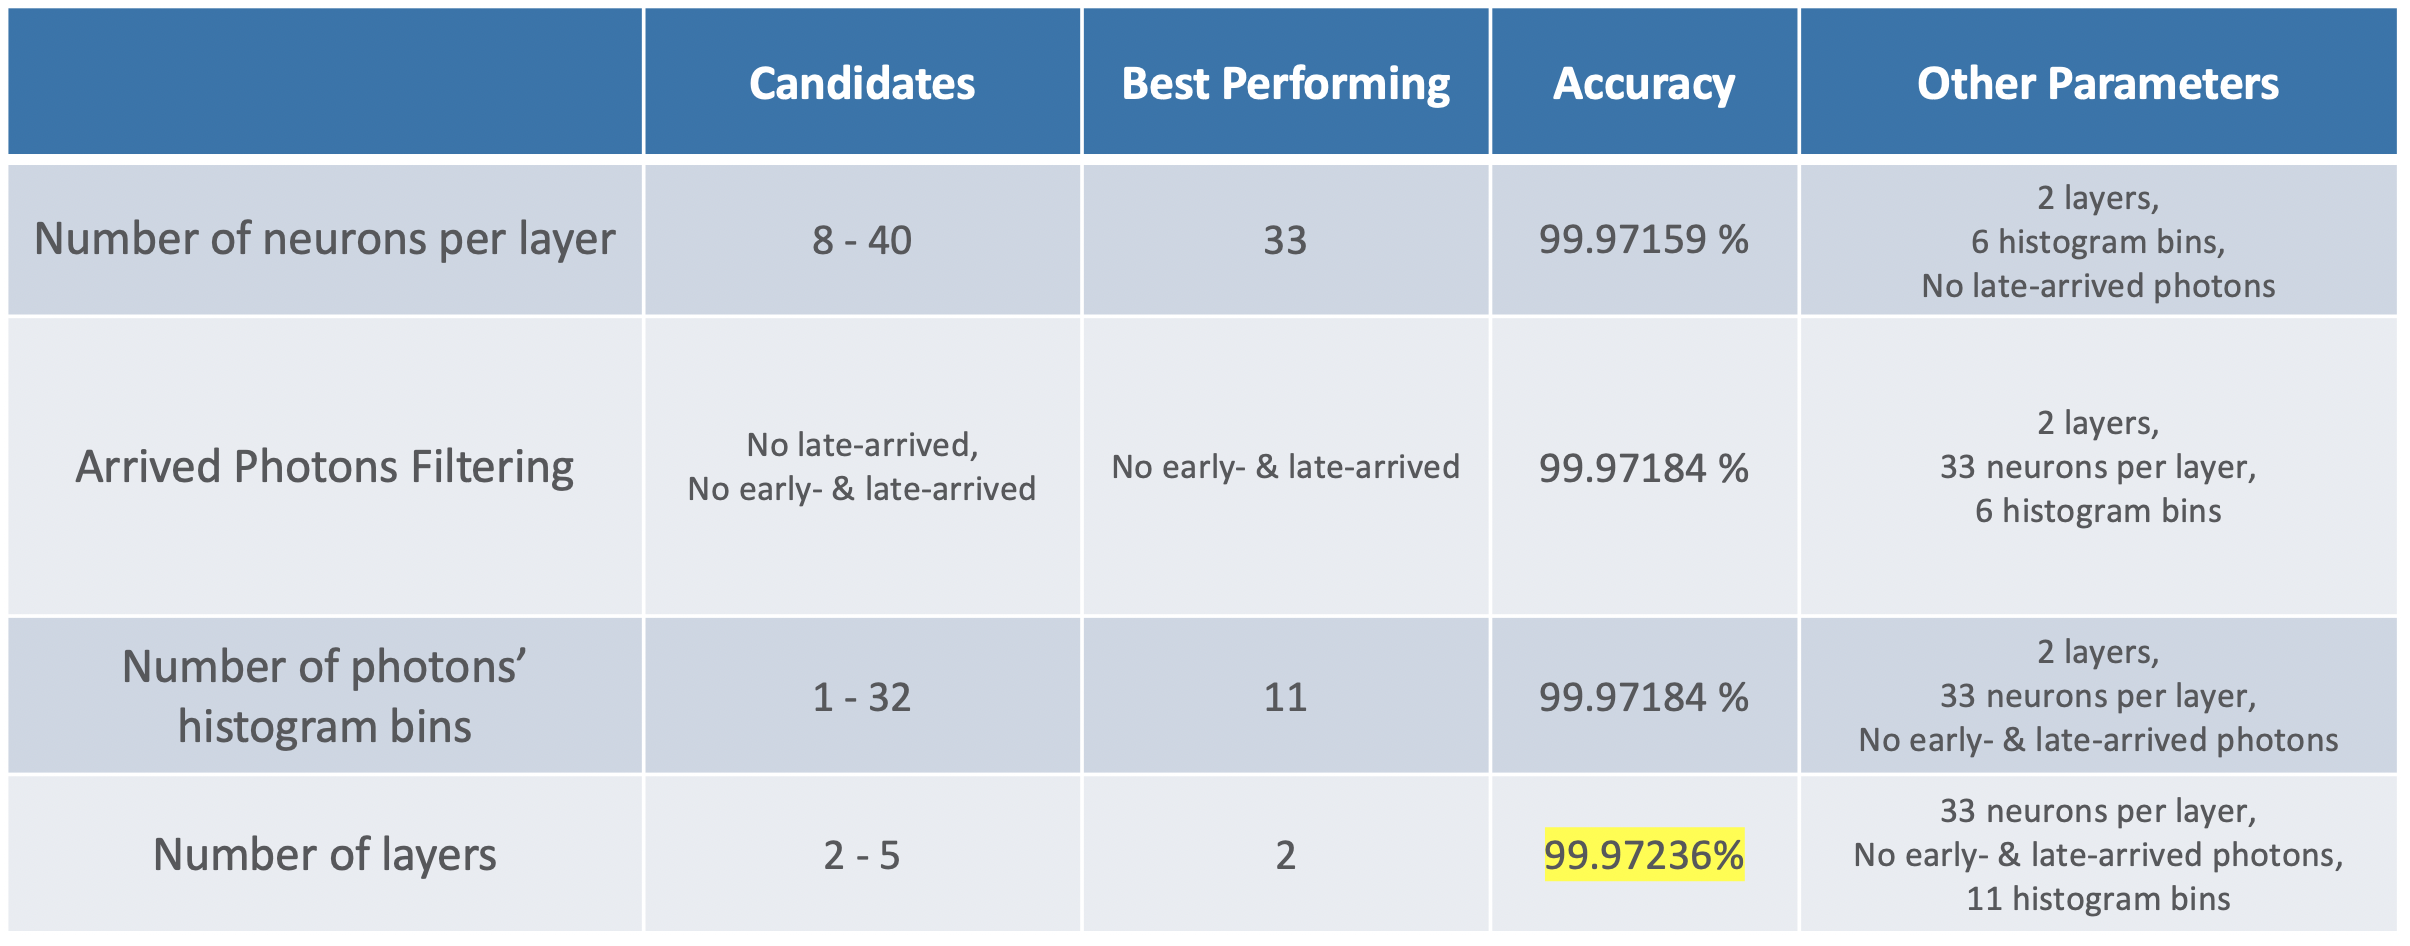
\includegraphics[width=2\columnwidth]{Figures/params_tuning.png}
    \centering
    \caption{Results of Hyper-parameters Tuning. Early-arrived photons refer to those arrived before $t = 0.722906$ ms; late-arrived photons refer to those arrived after $t = 5.22625$ ms.}
    \label{table:params_tuning}
\end{figure*}

\subsection{Ensemble Classifier}

The availability of multiple classification models explained in Section 3 and 4 motivates us to come up with a Voting Classifer: each individual classifier performs training and prediction individually, and the Voting Classifier takes a majority vote from all predictions as the final decision. We implemented such a Voting Classifier with three models: the Threshold Cutoff Model with Early-Arrived Photons, the Multilayer Perceptron and Linear Regression. The best set of hyper-parameters from previous evaluations are used in each individual model. Similar as above, the dataset is split properly and the Cross Testing Method is used for model evaluation. Interestingly, no significant performance improvement is observed in the Voting Classifier compared to each individual classifier. A deeper dive into the false positive and false negative instances demonstrate that every individual model tends to make mistakes on the same instances. Among all instances that are falsely-classified by at least one model, more than 75.2\% of those are misclassified by all three models. Therefore, using multiple classifiers to make a decision does not necessarily lead to a better performance, because these classifiers behave in a similar way and instances misclassified by one classifier tend to also be misclassified by all others with the same wrong label.

Figure \ref{fig:misclassified_photons_distro} and \ref{fig:misclassifed_photons_count} some properties of mis-classified instances by at least one classifier. The first graph shows a close-to-uniform distribution of all photons' arrival times; the second graph shows a counter-trend of the number of photons captured for a mis-classified qubit: a significant number of photons (with an average between 30 and 40) are captured for most Dark qubits so they're misclassified as Bright, and vice versa for most Bright qubits misclassified as Dark. Thus, it's expected that our current models are unable to classify those instances correctly because they don't follow the overall properties of the dataset. Figuring out a method to incorporate information in these misclassified instances into a classifier's training procedure is left as a topic of future research.

\begin{figure}[]
    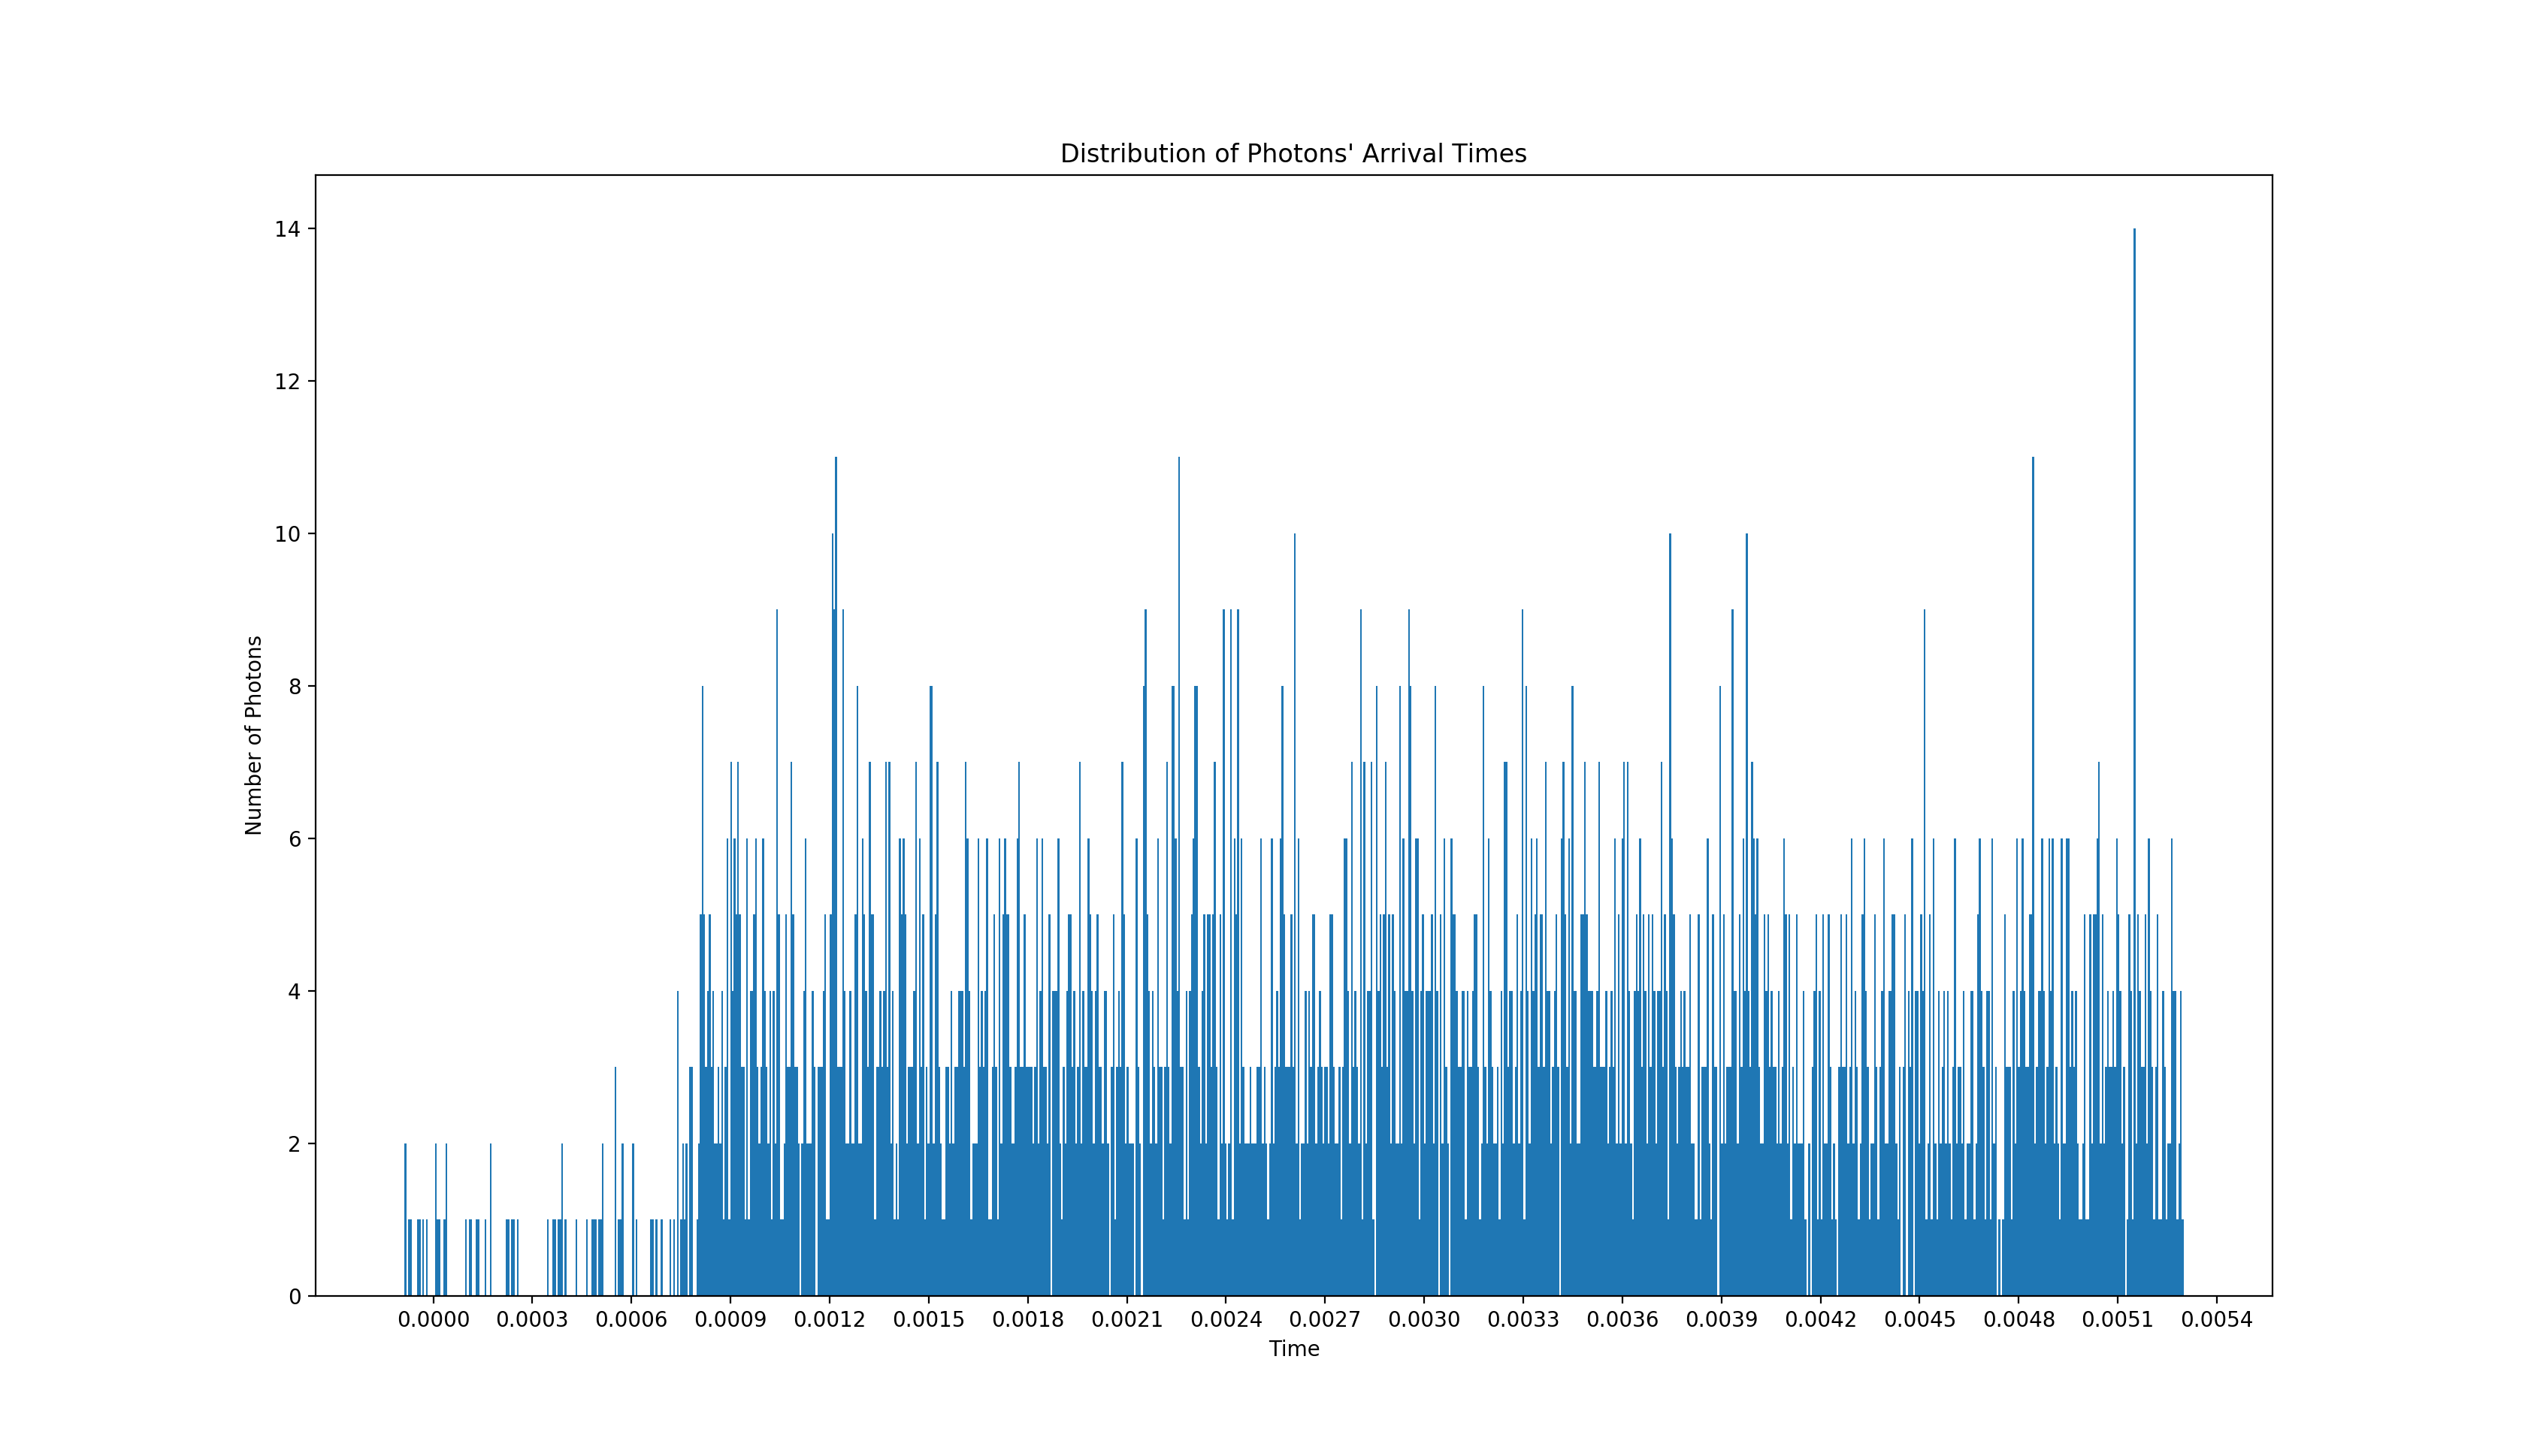
\includegraphics[width=\linewidth]{Figures/misclassified_photons_distro.png}
    \centering
    \caption{Distribution of photons' arrived times among misclassified qubit instances}
    \label{fig:misclassified_photons_distro}
\end{figure}

\begin{figure}[]
    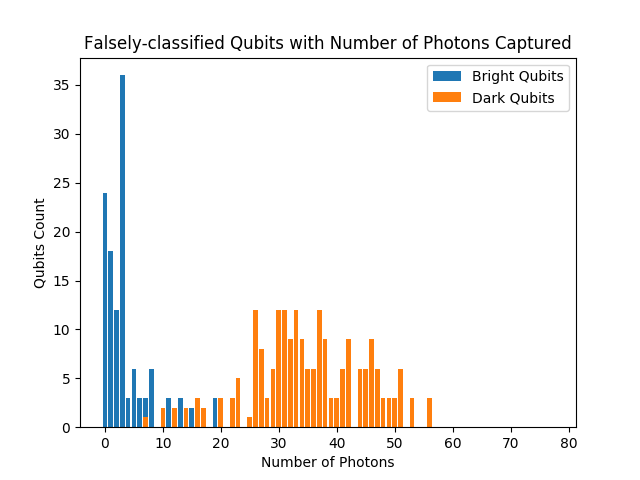
\includegraphics[width=\linewidth]{Figures/misclassifed_photons_count.png}
    \centering
    \caption{Qubits count for any particular number of photons captured, among misclassified qubit instances}
    \label{fig:misclassifed_photons_count}
\end{figure}

\section{Future Work}

Several potential approaches that are worth exploring to further increase the classification accuracy includes:

\begin{enumerate}
    \item 
    Account for the inaccurate ground truth labels in the dataset. All of the discussions above assume that the ground truth state is known for each qubit being measured. In fact, the accuracy of this ground truth may reside on the same order of magnitude as the accuracy of our classification models, so the former becomes a non-negligible error to consider during the model training and evaluation. Provided that it's not possible to obtrain higher-quality datasets in the near future, it may be beneficial to account for this inaccuracy with statistical models such as Bayesian statistics. 

    \item 
    Extract information of commonly misclassified instances and incorporate it into the training procedure of every model. For example, a new training procedure can be designed to always include all misclassified instances demonstrated in Section 6.2.

    \item 
    Approach the problem from a more scientific perspective rather than trial-and-error on machine learning models and parameter tunings. The performance may jump one level above if we are able to design a domain-specific model based on related quantum mechanics of the qubit operations.

\end{enumerate}

\section{Conclusion}

With the goal to improve measurement accuracy of a trapped-ion qubit, the problem can be framed as a binary classification problem and we have investigated multiple machine learning models as potential solutions, with a focus on the Multilayer Perceptron neural network model. With a careful input feature selection, data pre-processing and hyper-parameters tuning, the classification accuracy is improved from 99.97081\% in the baseline model to 99.97934\% with a random split of the training and testing set, which is about to reach the theoretical maximum reliability . A deeper dive into the dataset demonstrates the need of a fairer strategy to evaluate the model's accuracy and more constraints in the dataset splitting. With these new methods, the Multilayer Perceptron pipeline achieves accuracy at 99.97236\%, still an improvement over the baseline model. The better designed evaluation methods gain us confidence that this accuracy would persist in future datasets.

\section{Acknowledgement}

I greatly appreciate my academic advisor Jens Palsberg at UCLA Computer Science for introducing me to this project and guiding me through the entire research process. I greatly appreciate my teammates in the research group - Aaron Berdy, Akshay Utture, Ashwin Dharne, Shuyang Liu and Quentin Truong - for their valuable and inspiring suggestions on next steps through the research. Also, I greatly appreciate my friends and roommates Zeyuan Johnson Chen, Hao Jin, Jerry Tao, Senyang Jiang, Zhen Wang for patiently listening to my thoughts and help me learn the theories behind the statistical models. 

\begin{thebibliography}{9}
    \bibitem{ml-qubit} 
    Alireza Seif, Kevin A Landsman, Norbert M Linke, Caroline Figgatt, C Monroe and Mohammad Hafezi.
    \textit{Machine learning assisted readout of trapped-ion qubits}. 
    Journal of Physics B: Atomic, Molecular and Optical Physics. 2018.

    \bibitem{google-ai}
    \textit{IBM Research Blog}. 
    2019-10-22. Retrieved 2020-01-21.

    \bibitem{quantum-application}
    Jens Palsberg.
    \textit{UCLA CS-239 Spring 2019 Lecture Notes: Quantum Programming Foundations: History and Overview}.
    2019-03.

    \bibitem{fault-tolerance}
    Swamit Tannu.
    \textit{Towards Scalable and Reliable Architectures for Quantum Computing Platforms}.
    UCLA Faculty Candidate Talk. 2020-02-18.
\end{thebibliography}

\end{document}
